The results are based on simulations which are ran 10,000 times for each track. The total sum of crashes is 121,747.

\begin{tabularx}{.50\textwidth}{Xlllll}
country    & turn &mtr&brake  &speed &crashes\\
\hline
Australia  & R-L       & 381    &100    &150   &7837\\
China      & R-L       & 324.7  &50     &170   &7664\\
Bahrain    & R-L       & 476.4  &100    &70    &7792\\
Russia     & R-R       & 205.2  &-      &300   &2103\\
Spain      & R-L       & 690.5  &100    &130   &7211\\
Monaco     & R-R       & 111    &75     &103   &7477\\
Canada     & R-L       & 258    &125    &154   &6334\\
Azerbaijan & L-R       & 206    &50     &116   &7926\\
Austria    & R-L       & 318    &200    &122   &673\\
GB         & R-L       & 270    &-      &281   &991\\
Hungary    & R-L       & 576    &100    &85    &7550\\
Belgium    & R-L       & 251    &150    &77    &2887\\
Italy      & R-L       & 615    &125    &80    &7393\\
Singapore  & L-L       & 274    &50     &126   &8724\\
Malaysia   & R-L       & 620    &100    &74    &8849\\
Japan      & R-L       & 373    &10     &152   &1262\\
USA        & L-R       & 364    &100    &86    &8217\\
Mexico     & R-L       & 890    &200    &107   &6279\\
Brazil     & L-R       & 334    &50     &109   &5129\\
UAE        & L-R       & 305    &50     &150   &9449\\
\end{tabularx}
\captionof{table}{Overview of grand prix, with circuit data.}\label{table:results}

All the circuits are listed in table \ref{table:results}, with all the necessary data. In the last column we can see the numbers of crashes based om our simulation model. The number of crashes seems divided equally for most of the circuits. Some of them have significant lower crashes, e.g. Austria, with only 673 crashes.

\begin{tikzpicture}
\begin{axis}[
  title={brake distance, crashes},
  xlabel={brake distance},
  ylabel={crashes},
  ymajorgrids=true,
  grid style=dashed,
]
\addplot[ only marks ]
  coordinates {(0,991)(0,2103)(10,1262)(25,7477)(50,7926)(50,5129)(50,7664)(50,8724)(50,9449)(100,7837)(100,7792)(100,7550)(100,8849)(100,7211)(100,8217)(125,6334)(125,7393)(150,2887)(200,673)(200,6279)};
  \addplot [thick, red] table[y={create col/linear regression}]{
    0 991
    0 2103
    10 1262
    25 7477
    50 7926
    50 5129
    50 7664
    50 8724
    50 9449
    100 7837
    100 7792
    100 7550
    100 8849
    100 7211
    100 8217
    125 6334
    125 7393
    150 2887
    200 673
   };
\end{axis}
\end{tikzpicture}
\captionof{figure}{Crashes on scale of brake distance}\label{fig:results1}

In figure \ref{fig:results1} every single dot means the numbers of crashes based on the brake distance. In this figure we see a stable trend. It seems that the brake distance doesn't affect the number of crashes.

\begin{tikzpicture}
\begin{axis}[
  title={distance, crashes},
  xlabel={distance},
  ylabel={crashes},
  ymajorgrids=true,
  grid style=dashed,
]
\addplot[ only marks ]
  coordinates {(111,7477)(205.2,2103)(206,7926)(251,2887)(258,6334)(270,991)(274,8724)(305,9449)(318,673)(324.7,7664)(334,5129)(364,8217)(373,1262)(381,7837)(476.4,7792)(576,7550)(615,7393)(620,8849)(690.5,7211)(890,6279)};
  \addplot [thick, red] table[y={create col/linear regression}]{
    111 7477
    205.2 2103
    206 7926
    251 2887
    258 6334
    270 991
    274 8724
    305 9449
    318 673
    324.7 7664
    334 5129
    364 8217
    373 1262
    381 7837
    476.4 7792
    576 7550
    615 7393
    620 8849
    690.5 7211
    890 6279
  };
\end{axis}
\end{tikzpicture}
\captionof{figure}{Crashes on scale of turn distance}\label{fig:results2}

According to figure \ref{fig:results2}, we see that the number of crashes increase when the distance rises. There are numerous causes for this, high speed could be one.

\begin{tikzpicture}
\begin{axis}[
  title={speed, crashes},
  xlabel={speed},
  ylabel={crashes},
  ymajorgrids=true,
  grid style=dashed,
]
\addplot[ only marks ]
  coordinates {(70,7792)(74,8849)(77,2887)(80,7393)(85,7550)(86,8217)(103,7477)(107,6279)(109,5129)(116,7926)(122,673)(126,8724)(130,7211)(150,7837)(150,9449)(154,6334)(170,7664)(252,1262)(281,991)(300,2103)};
  \addplot [thick, red] table[y={create col/linear regression}]{
    70 7792
    74 8849
    77 2887
    80 7393
    85 7550
    86 8217
    103 7477
    107 6279
    109 5129
    116 7926
    122 673
    126 8724
    130 7211
    150 9449
    150 7837
    154 6334
    170 7664
    252 1262
    281 991
    300 2103
  };
\end{axis}
\end{tikzpicture}
\captionof{figure}{Crashes on scale of turn speed}\label{fig:results3}

When a driver can take a turn without braking much, the number of crashes will decrease. Figure \ref{fig:results3}
is a nice description of this behaviour and it seems logical. Imagine that you have a large turn coming ahead, then you and the drivers in front of you don't have to brake suddenly.

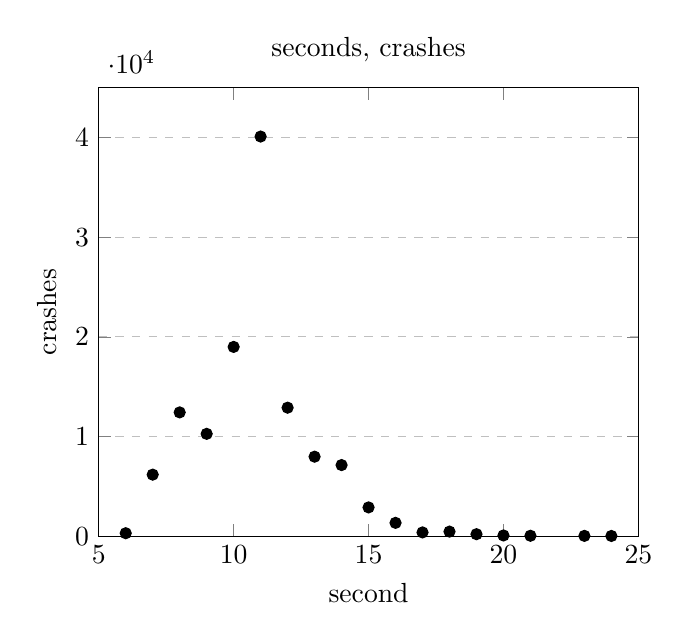
\begin{tikzpicture}
\begin{axis}[
  title={seconds, crashes},
  xlabel={second},
  ylabel={crashes},
  xmin=5, xmax=25,
  ymin=0, ymax=45000,
  ymajorgrids=true,
  grid style=dashed,
]
\addplot[ only marks ]
  coordinates {(6,297)(7,6177)(8,12426)(9,10272)(10,18999)(11,40115)(12,12898)(13,7980)(14,7137)(15,2888)(16,1338)(17,378)(18,458)(19,200)(20,73)(21,42)(23,31)(24,21)(28,17)};
\end{axis}
\end{tikzpicture}
\captionof{figure}{Crashes on scale of seconds}\label{table:results}


\begin{tikzpicture}
\begin{axis}[ title={metres in Monaco, crashes}, xlabel={metres}, ylabel={crashes}, xmin=75, xmax=125, ymin=0, ymax=1000, ymajorgrids=true, grid style=dashed, ]
\addplot[ only marks ]
  coordinates {(79,19)(83,21)(84,20)(91,194)(92,106)(93,235)(94,277)(95,452)(96,150)(99,960)(100,867)(101,297)(102,504)(103,1618)(104,36)(105,144)(107,339)(108,241)(109,324)(110,673)};
\addplot [thick, red] table[y={create col/linear regression}]{
    79 19
    83 21
    84 20
    91 194
    92 106
    93 235
    94 277
    95 452
    96 150
    99 960
    100 867
    101 297
    102 504
    103 1618
    104 36
    105 144
    107 339
    108 241
    109 324
    110 673
  };
\end{axis}
\end{tikzpicture}


\begin{tikzpicture}
\begin{axis}[ title={metres in Mexico, crashes}, xlabel={metres}, ylabel={crashes}, ymajorgrids=true, grid style=dashed, ]
\addplot[ only marks ]
  coordinates {
(201,292)(205,300)(214,321)(317,320)(480,332)(496,286)(505,543)(512,131)(517,313)(537,475)(541,160)(590,173)(592,158)(605,334)(661,601)(693,71)(697,77)(700,332)(708,219)(729,80)(733,46)(746,146)(750,148)(770,35)(788,74)(810,152)(857,22)(886,138)
};
  \addplot [thick, red] table[y={create col/linear regression}]{
    201 292
    205 300
    214 321
    317 320
    480 332
    496 286
    505 543
    512 131
    517 313
    537 475
    541 160
    590 173
    592 158
    605 334
    661 601
    693 71
    697 77
    700 332
    708 219
    729 80
    733 46
    746 146
    750 148
    770 35
    788 74
    810 152
    857 22
    886 138
  };
\end{axis}
\end{tikzpicture}

\begin{tikzpicture}
\begin{axis}[ title={metres in Bahrain, crashes}, xlabel={metres}, ylabel={crashes}, ymajorgrids=true, grid style=dashed, ]
\addplot[ only marks ]
  coordinates {
  (201,305)(205,327)(214,314)(317,295)(391,18)(392,162)(395,298)(407,185)(411,41)(418,292)(423,233)(427,89)(431,380)(433,502)(434,1)(435,3)(441,141)(443,52)(444,301)(447,502)(449,20)(450,129)(453,161)(454,3)(455,897)(458,11)(460,321)(461,308)(466,580)(467,316)(471,454)(473,74)(474,77)
};
  \addplot [thick, red] table[y={create col/linear regression}]{
    201 305
    205 327
    214 314
    317 295
    391 18
    392 162
    395 298
    407 185
    411 41
    418 292
    423 233
    427 89
    431 380
    433 502
    434 1
    435 3
    441 141
    443 52
    444 301
    447 502
    449 20
    450 129
    453 161
    454 3
    455 897
    458 11
    460 321
    461 308
    466 580
    467 316
    471 454
    473 74
    474 77
  };
\end{axis}
\end{tikzpicture}

    (205,327)(214,314)(317,295)(391,18)(392,162)(395,298)(407,185)(411,41)(418,292)(423,233)(427,89)(431,380)(433,502)(434,1)(435,3)(441,141)(443,52)(444,301)(447,502)(449,20)(450,129)(453,161)(454,3)(455,897)(458,11)(460,321)(461,308)(466,580)(467,316)(471,454)(473,74)(474,77)
